% Le standard IIIF

\subsection{IIIF et les données ouvertes}
    \subsubsection{Principes et objectifs}
	Le standard \iiif\footcite{IIIFInternationalImage} est une initiative collaborative lancée en 2011 par un groupement d'institutions\footnote{Les collaborateurs à l'initiative du projet sont la British Library, la \bnf, Stanford University, les Bodleian Libraries, la Bibliothèque nationale de Norvège, la Bibliothèque nationale de Los Alamos et Cornell University.} attachées à faciliter la diffusion sur le Web des ressources iconographiques des collections patrimoniales \footcite{cramerInternationalImageInteroperability2011}. La volonté de développement de ce standard provient du constat que, malgré la nécessité d'un accès global aux images numériques pour la transmission du patrimoine culturel, un grand nombre de ces ressources restent, sur Internet, isolées dans des silos d'informations dont l'accès n'est possible que par des applications spécifiques à chaque institution\footcite{cramerInternationalImageInteroperability2011}, rendant complexe le partage et la mise en commun des ressources.
	
	De cette observation est née la volonté de créer un outil proposant des méthodes standardisées de partage sur le Web des images et de leurs métadonnées, pour toute institution qui souhaiterait partager numériquement ses collections. \iiif propose ainsi un standard dont les fonctionnalités vont au-delà de celles d'un navigateur, capable d'afficher des formats libres d'image\footnote{\iiif propose également, depuis 2020, un service dédié aux fichiers vidéo, que nous n'abordons pas dans ce mémoire car les projets étudiés portent tous sur des images fixes.}, sans proposer plus d'interaction avec les images servies\footcite{HowItWorks}. \iiif propose ainsi des outils interopérables, libres d'accès, permettant notamment de zoomer en profondeur sur les images, d'y appliquer des traitements visuels simples, de reconstruire la structure du document ou de les annoter.
	
	Pour assurer ces fonctionnalités, \iiif s'appuie sur deux \api\footnote{Une \api est une interface logicielle permettant de connecter entre eux des logiciels pour échanger des données, des fonctionnalités ou des services.} : l'\api Image et l'\api Présentation. Ces \api sont le socle du standard, elles en assurent la cohérence afin que les images puissent être partagées de manière fluide entre les institutions et projets. Le cœur du standard \iiif, qui fait tout son intérêt dans le contexte décrit précédemment du partage des images sur le Web, est en effet l'interopérabilité : \iiif assure ainsi la portabilité entre les visualiseurs, pour permettre une transmission réellement fluide de l'information.
    
    \subsubsection{Les API IIIF}
	Le fonctionnement du standard \iiif s'appuie sur deux éléments essentiels : l'envoi des images depuis les serveurs, et leur visualisation. 
	
	L'\api Image définit les spécifications pour un service renvoyant une image en réponse à une requête \http ou \https : à partir d'une \uri valide, l'image peut être affichée dans un visualiseur, ou dans un navigateur. L'\uri peut spécifier, dans sa requête, la région, la taille, la rotation, la qualité ou le format de l'image demandée, suivant des instructions spécifiques prédéfinies par le standard\footcite{ImageAPI}. En ajustant les paramètres, l'utilisateur peut ainsi obtenir une image qu'il peut modifier en accord avec ses besoins sans passer par un éditeur spécifique. L'\api Image, développée pour des clients tels que les applications d'institutions patrimoniales, peut être implémentée sans l'\api Présentation : seule, elle permet notamment un zoom rapide et profond sur des images en très haute résolution.
	
	L'\api Présentation permet d'introduire des fonctionnalités plus vastes en termes d'informations liées aux images : par le biais d'un manifeste au format \json, elle attache aux images des métadonnées descriptives, administratives et structurelles qui définissent la manière dont elles seront présentées dans un visualiseur. Le manifeste permet notamment de rassembler en un fichier les différents éléments d'un objet \iiif\footcite{HowItWorks}, et notamment les séries d'images\footnote{Cette fonctionnalité est particulièrement intéressante pour les numérisations d'ouvrages, puisqu'elle permet de regrouper en un fichier toutes les pages numérisées.}, tout en gérant également leur ordre dans le document numérique. Le manifeste contient généralement des informations d'identification de l'objet original\footnote{On retrouve notamment le titre, l'auteur, l'institution de conservation, le numéro d'inventaire ou la cote, et les informations sur les droits de diffusion.}, et peut être enrichi d'annotations sur l'objet ou son contenu\footcite{PresentationAPI}.
	
	Pour afficher les images et les informations liées, il existe une multitude de visualiseurs\footcite{IIIFViewers} aux fonctionnalités différentes, tous compatibles avec tous les manifestes \iiif, quelle que soit leur institution d'origine. Ainsi, les ressources produites par les institutions peuvent être consultées par le biais d'outils libres, accessibles à tous. Pour aller au-delà des fonctionnalités proposées par les deux \api centrales du standard, quatre autres \api ont été développées, pour gérer d'autres besoins liés à mise à disposition d'images tout en respectant des principes standardisés\footcite{HowItWorks}.
    
    \subsubsection{Anatomie d'un manifeste}
	Pour constituer les éléments retournés par les \api \iiif, il existe un modèle de données spécifique, qui assure la caractérisation des objets selon des normes communes, qui permettent de conserver l'interopérabilité du standard. Il existe ainsi des types de ressources, ou classes, précisément définies, avec une hiérarchie fixe (fig. \ref{fig:iiif_data_model}), qui permettent de décrire les objets numérisés au format \json.
	
	Un manifeste est un fichier au format \json. Du point de vue de la donnée, la classe \textit{Manifest} permet de décrire un objet composé, une œuvre dans sa totalité : elle contient ainsi un ensemble de métadonnées descriptives la concernant (titre, auteur, institution de conservation, licence), et permet, si nécessaire, de reconstituer la structure de l'objet à partir des \textit{Canvases}.
	
	Le \textit{Canvas} est un conteneur de niveau inférieur au \textit{Manifest}, qui permet de représenter une vue spécifique d'un objet, et les métadonnées qui y sont associées. Si nécessaire, un élément de niveau supérieur peut exister entre les \textit{Canvases} et le \textit{Manifest} : il s'agit des \textit{Ranges}, qui permettent de décrire une séquence de \textit{Canvases}.
	
	Il existe, à un niveau supérieur au \textit{Manifest}, une classe \textit{Collection}, qui assure une plus grande flexibilité du modèle pour les projets qui souhaiteraient réunir plusieurs objets dans une catégorie plus large. Une \textit{Collection} peut représenter une liste de \textit{Manifests}, ou une liste de \textit{Collections}, permettant ainsi de regrouper des objets ou groupes d'objets selon un cadre défini, qui facilite la navigation dans un ensemble restreint de ressources liées\footcite{PresentationAPI}.
	
	Pour un manifeste ne contenant que des images et leurs métadonnées, ces éléments suffisent à construire un fichier cohérent et fonctionnel, qui pourra être lu par un visualiseur \iiif.
	
	Pour annoter les images d'un manifeste, il existe une série de types de ressource additionnels qui contiennent les annotations selon une hiérarchie précise, et les rattache à un \textit{Canvas} spécifique. L'\textit{Annotation Page} contient une liste ordonnée d'\textit{Annotations} pour un \textit{Canvas} : pour annoter un manifeste, il existe donc autant d'\textit{Annotation Pages} qu'il existe de \textit{Canvases} annotés.
	
	La classe \textit{Annotation} fait le lien entre le contenu de l'annotation (\textit{Content}) et le \textit{Canvas}\footcite{PresentationAPI} : ce type de ressource permet d'assurer l'interopérabilité du modèle, puisqu'elle permet l'alignement des annotations et des images, y compris dans le contexte d'annotations produites par un utilisateur différent du créateur du manifeste. Ainsi, ce modèle de données permet la collaboration entre plusieurs utilisateurs à partir d'un manifeste produit par une institutions, et rend possible la réutilisation des images comme des manifestes dans des projets ultérieurs, avec la fluidité d'un modèle partagé, standard, qui ne nécessite aucun effort d'alignement entre institutions.
	
	\begin{figure}[h]
		\centering
		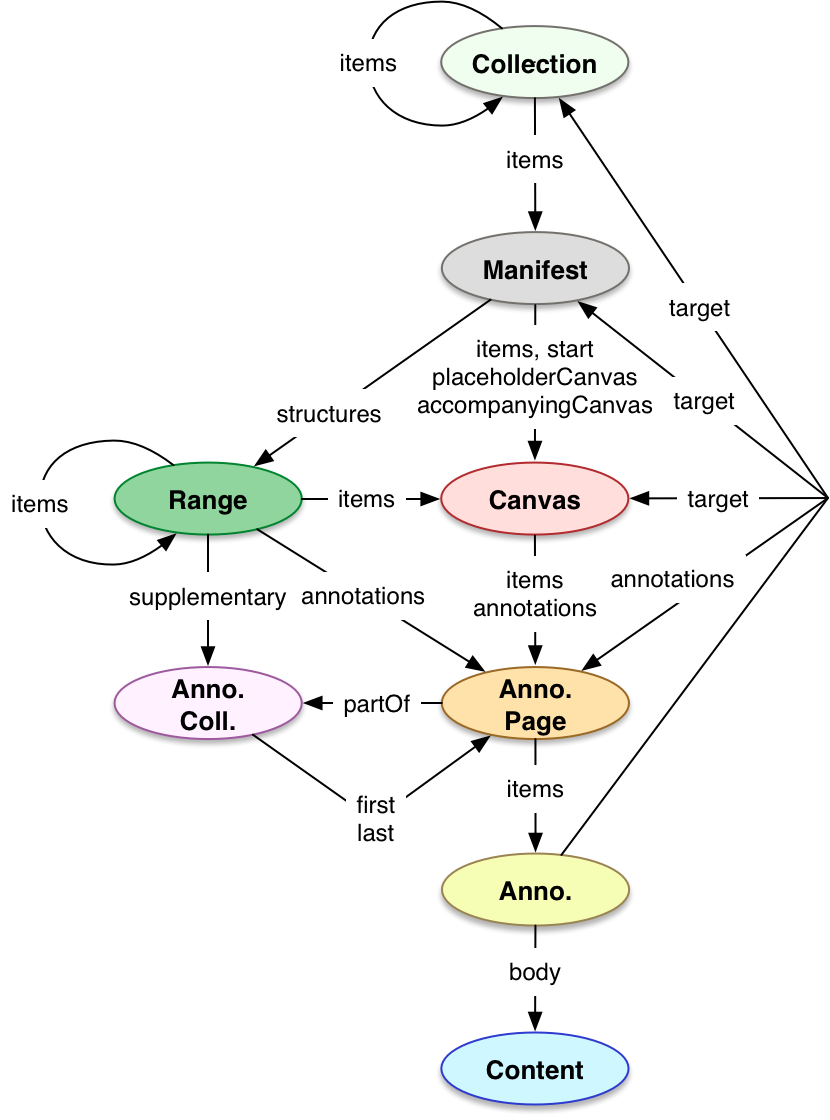
\includegraphics[width=10cm]{images/modele_donnees_iiif.png}
		\caption{Modèle de données \iiif pour la description d'un objet}
		\label{fig:iiif_data_model}
	\end{figure}
    
\subsection{IIIF, un modèle universel ?}
    \subsubsection{Limites de l'interopérabilité du standard}
	\iiif est ainsi pensé comme un standard universel permettant aux institutions et aux projets qui le souhaitent de partager leurs ressources, de les mettre à disposition en assurant la possibilité de leur réutilisation : dans une optique de science ouverte, \iiif permet de partager aisément les résultats de projets de recherche impliquant des images.
	
	Cependant, malgré l'existence d'un modèle de données standard pour la description des objets, \iiif présente des limites dans son universalité. En effet, malgré son cadre construit pour assurer l'interopérabilité des manifestes, le modèle n'est en pratique pas employé de la même manière par toutes les institutions, et nécessite donc une adaptation des développements faits autour de \iiif pour prendre en compte ces exceptions. Nous constatons, par exemple, que si les ressources images sont supposées être intégrées au manifeste dans un conteneur \textit{Canvas}, certaines institutions -- comme la bibliothèque univeristaire de Yale -- utilisent plutôt des \textit{Items} (fig. \ref{fig:manifests_canvas}), modifiant ainsi profondément la structure du manifeste \iiif tout en conservant un fichier lisible par les visualiseurs. L'application du standard varie ainsi d'une institution à l'autre, sans altérer le fonctionnement des outils de base de \iiif, mais en provoquant cependant une déperdition de son universalité pour des projets qui souhaiteraient développer des outils autour de ces manifestes. 
	
	Dans un projet reposant sur l'exploitation d'images d'objets patrimoniaux, tels que les projets décrits dans ce mémoire, il est ainsi nécessaire de prendre en compte ces exceptions techniques : dans le cadre du projet \eida, la récupération des images est effectuée par un algorithme spécifique\footcite{albouyIiifdownloader2023}, qui parse un manifeste \iiif déposé par un utilisateur dans l'application du projet et en extrait des fichiers images pour les enregistrer. Dans le développement de cet algorithme, il a ainsi été nécessaire de prendre en compte les exceptions possibles, pour ne pas créer d'erreur en cas de dépôt d'un manifeste à la structure différente.

	\begin{figure}[h]
		\begin{subfigure}{1\linewidth}
			\centering
			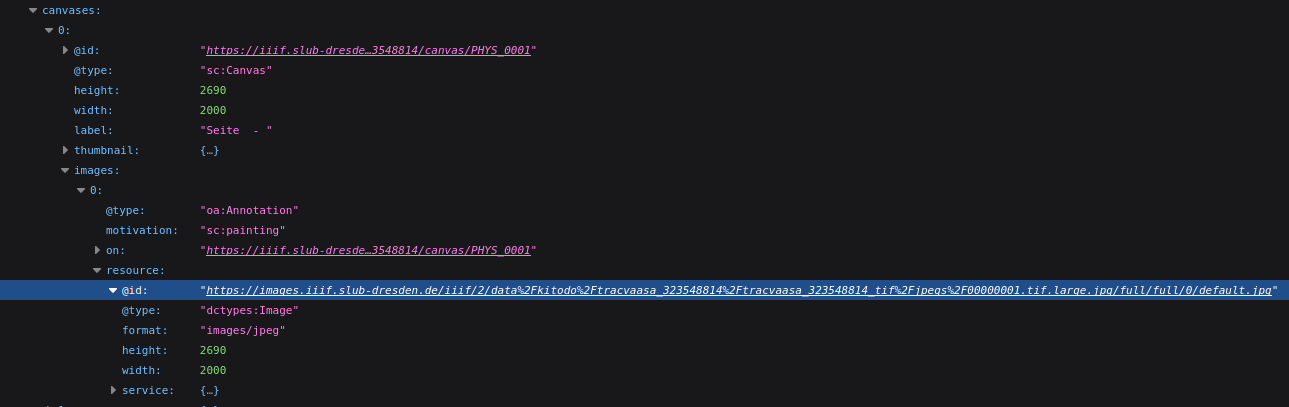
\includegraphics[width=15cm]{images/dresden_manifest.png}
			\subcaption{Manifeste \iiif de la bibliothèque universitaire de Dresde avec \textit{Canvases}}
		\end{subfigure}
		\hspace{1pt}
		\begin{subfigure}{1\linewidth}
			\centering
			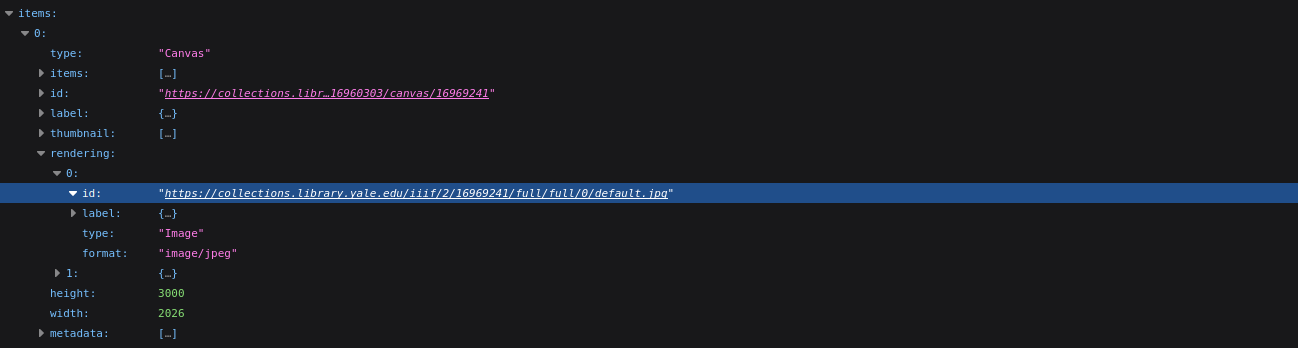
\includegraphics[width=15cm]{images/yale_manifest.png}
			\subcaption{Manifeste \iiif de la bibliothèque universitaire de Yale avec \textit{Items}}
		\end{subfigure}
		\hspace{1pt}
		\caption{Comparatif des ressources contenant les images de deux manifestes \iiif}
		\label{fig:manifests_canvas}
	\end{figure}

    \subsubsection{Implémentation de IIIF : un réflexe global ?}
	Pour les projets de recherche exploitant des images respectant le standard \iiif, il se pose la question des institutions ayant fait le choix de gérer leurs images différemment. En effet, si de nombreuses institutions ont adopté le standard et mis en ligne des centaines de millions d'images compatibles depuis la naissance de l'initiative\footcite{malloryIIIFMuseumsExplained2019}, il n'est ni obligatoire ni systématique, et il reste ainsi un nombre certain d'établissements qui gèrent leurs images avec des outils techniques différents, et restent ainsi exclus du standard. Les musées, notamment, et particulièrement les musées hors Amérique du Nord, exploitent encore peu les possibilités offertes par \iiif en termes de partage des images\footcite{IIIFMuseumsFrance2023}, et restent en marge de cette initiative de facilitation de la mise en commun et de l'exploitation des ressources iconographiques.
	
	Il n'est cependant pas envisageable, dans le cadre d'un projet de recherche, d'exclure totalement les sources provenant d'institutions n'utilisant pas le standard \iiif : il est donc nécessaire, dans le développement d'outils numériques pour la gestion des images, de prendre en compte ces sources aux formats différents, qu'il faut traiter pour les rendre exploitable de la même manière que le sont les images extraites de manifestes \iiif. Ainsi, dans la chaîne de traitement des images, une réflexion doit être menée pour l'intégration d'autres formats, tels que les PDF pour les numérisations d'ouvrages, ou les fichiers images indépendants. Malgré la fluidité du traitement des sources permise par l'existence d'un standard, il est ainsi nécessaire de réfléchir à des solutions techniques au-delà des limites de ce dernier, pour ne pas exclure des corpus les sources numérisées présentant un intérêt pour la recherche. 
	
	Dans un projet de recherche en vision artificielle, l'utilisation du standard \iiif permet, d'une part, la constitution aisée d'un corpus d'images, qu'il est possible de récupérer directement sur les sites des institutions à l'aide des \api : le standard \iiif fluidifie fortement les échanges et la réutilisation des documents numérisés, et permet de construire un outil générique pour le traitement de sources numériques provenant d'institutions diverses. Il reste cependant de nombreux cas où une chaîne de traitement parallèle doit être développée, pour pallier à l'absence d'implémentation du standard dans certaines institutions. D'autre part, l'utilisation du standard \iiif pour la publication en ligne des données du projet permet également d'envisager leur réutilisation future par d'autres initiatives, en s'assurant de l'interopérabilité des résultats produits, dans une démarche de science ouverte.
